\documentclass{article}
\usepackage[utf8]{inputenc}
\usepackage[english, science, small]{ku-frontpage}
\usepackage{tabularx}

\title{Software Engineering: First hand in}
\subtitle{}
\assignment{First hand in}
\author{Matias Korn(crd551), Samuel Korn(rxq534), Nikolin Prenga (hpq143), Silvan Adrian (zlp432)}
\advisor{}
\date{February 2019}

\begin{document}

\maketitle

\section{Solution and problem domain}
Citizens have the possibility to apply for loss of earnings. Loss of earnings means, that the earnings the citizen has missed out on, due to being occupied of taking care of a child. There are many actors involved when the citizen apply for loss of earnings. First off, there is the case-worker, who receives the application from the citizen. The case-worker is working at a municipality council. The municipality council has to comply with the law and paragraph 42 and the rules that are provided from the ministry of social affairs.

The ministry of social affairs lay down the rules of:
(1) How big a possible cap of allowed compensation is.
(2) How much the pension scheme is obligated to contribute with. (3) How the calculation of the actual compensation is made. (4) What the limit is of how much the pension scheme is obligated to contribute with. (5) How much of the loss on the pension contribution shall be paid by the receiver and municipal council.

As mentioned, the case-workers handles the cases and receives all the necessary information, for complying with paragraph 42. First of, the case-worker has to establish, if there are grounds for compensation. (1) The child has to be under 18. (2) The conditions on the child's health have to abide by the law, for that the child's health record has to be collected from the health care system. The health record has to confirm, that it is most expedient for the mother or father to the care of the child, at home or has been placed in care under section 52(3)(vii). If that is the case, the condition is, that it is most expedient for a parent to be there. It might be difficult to establish, if that is the case, based on the health record, if it is not explicitly stated, therefore it might be necessary to collect a confirmation by the child's doctor. (3) Loss of income has to be established, for that the necessary bank statements have to be provided.

Our solution is concerned with case management. We have to provide a platform for collecting, recording the progress and the final decisions that have been made and what grounds there has been for them. The following actors are directly involved in our system: (1) the citizen, (2) the case-worker, (3) the minister of social affairs(external system), (4) the law that decides if the citizen is permitted for loss of earnings, (5) the payment system(external system), that is available for the municipal council. Our solutions will handle the information gathering. Storing the information relevant for the case. The final decision whether or not the citizen has been granted compensation and calculating the amount granted for payout to both the citizen and pension scheme, based on the numbers provided by the minister of social affairs.

\section{Scenarios}

- Case with parents apply for loss of earnings.

- case with municipality receiving possible loss of earnings from hospital and needs to get processed.

\subsection{Scenario 1 - Application from parent(s)}
\begin{enumerate}
    \item Parent is making an application.
    \item Case-worker is validating the application.
        \begin{enumerate}
            \item The case-worker is confirming that the doctor confirmation is not falsified.
            \item The case-worker is confirming that the required payslip is provided and not falsified. 
            \item The case-worker is confirming that the required pension-scheme contract is provided and not falsified.
        \end{enumerate}
    \item Case-worker is documenting and archiving all the provided information. 
    \item Case-worker is accepting the application. 
    \item Case-worker send response about the outcome of the application.
    \item Case-worker send off the amount and the amount of months for payout to the payment system. 
\end{enumerate}

\subsection{Scenario 2 - Application with additional requests}

\subsection{Scenario 3 - Receiving information from the hospital}

\section{functional requirements}

\section{Non-functional requirements}

Note (Matias): fault tolerant system for secure and stable persisting.

\section{Use case diagram}

% to do: extend

\begin{figure}[htb!]
	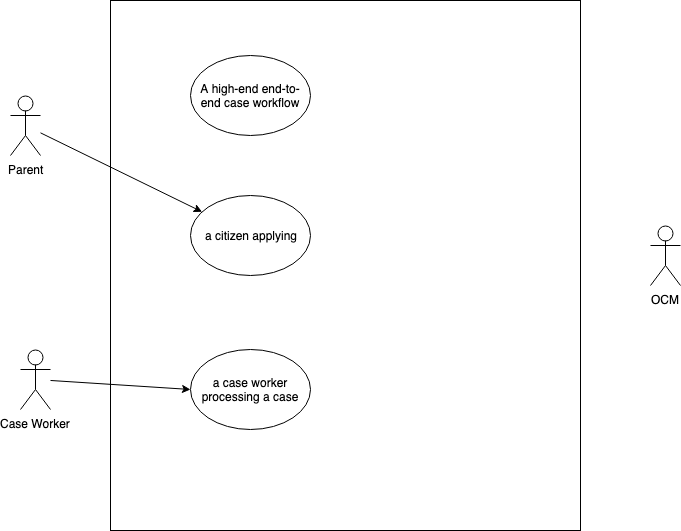
\includegraphics[width=\textwidth]{img/use-cases}
\end{figure}


\section{Detailed Use cases}

\subsection{UC01: A high-end end-to-end case workflow}

\begin{tabularx}{\textwidth}{l|l}
	\textbf{Use Case name} & A high-end end-to-end case workflow \\
	\hline
	\textbf{Participating actor} & \\
	\hline
	\textbf{Flow of events} &
	\begin{minipage}{\linewidth}
		\begin{enumerate}
			\item asds
			\item asdasdasds
		\end{enumerate} 
	\end{minipage}\\
	\hline
	\textbf{Entry condition} & \\
	\hline
	\textbf{Exit condition} & \\
	\hline
	\textbf{Quality requirements} & \\
\end{tabularx}



\subsection{UC02: A citizen applying}

\begin{tabularx}{\textwidth}{l|l}
	\textbf{Use Case name} & A high-end end-to-end case workflow \\
	\hline
	\textbf{Participating actor} & \\
	\hline
	\textbf{Flow of events} & \\
	\hline
	\textbf{Entry condition} & \\
	\hline
	\textbf{Exit condition} & \\
	\hline
	\textbf{Quality requirements} & \\
\end{tabularx}

\subsection{UC03: A case worker processing a case}
\begin{tabularx}{\textwidth}{l|l}
	\textbf{Use Case name} & A high-end end-to-end case workflow \\
	\hline
	\textbf{Participating actor} & \\
	\hline
	\textbf{Flow of events} & \\
	\hline
	\textbf{Entry condition} & \\
	\hline
	\textbf{Exit condition} & \\
	\hline
	\textbf{Quality requirements} & \\
\end{tabularx}

\subsection{UCX: ...}

\section{Architecture model}


\section{Project plan}

\subsection{Team composition/roles}
\textbf{Silvan Adrian}
\begin{itemize}
	\item SCRUM Master %otherwise won't make much sense of having a project team without a scrum master
\end{itemize}
\textbf{Matthias Korn}
\begin{itemize}
	\item Developer
\end{itemize}
\textbf{Samuel Korn}
\begin{itemize}
	\item Developer
\end{itemize}
\textbf{Nikolin Prenga}
\begin{itemize}
	\item Developer
\end{itemize}

\subsection{Skill matrice}
%fill up
\begin{table}[htb!]
\begin{tabular}{lllll}
 \textbf{Skill}  & \textbf{Silvan} & \textbf{Matthias} & \textbf{Jonathan} & \textbf{Nikolin} \\
\hline
Development       &                 &                   &                   &                  \\
Project Management &                 &                   &                   &                  \\
                  &                 &                   &                   &                 
\end{tabular}
\end{table}

\subsection{Work Packages}
% just a graph or actually some coding involved?

\subsection{Schedule}
As the project methodology SCRUM will be used, so after each Sprint there will be  working increment released.


\begin{table}[htb!]
\begin{tabular}{lll}
\textbf{Sprint} & \textbf{Sprint Goal} & \textbf{Date} \\
\hline
1      & Set Up Infrastructure & xx.xx \\
2      & Do more etc.          &            \\
3       &                       &           
\end{tabular}
\end{table}

\subsection{Risks}

\begin{tabularx}{\textwidth}{llllXX}
\textbf{Nr} & \textbf{Description} & \textbf{Probability} & \textbf{Criticality} & \textbf{Prevention}                                                      & \textbf{Measure}                                                                             \\
\hline
R1          & Worker gets sick     & 10\%                 & high                 & Every worker should be able to replace the skill of an other in the team & Split up work not only according to someones skills but also to get them to learn new things \\
            &                      &                      &                      &                                                                          &                                                                                              \\
            &                      &                      &                      &                                                                          &                                                                                             
\end{tabularx}


\end{document}
